%
\section{Sorting Algorithms}

It is common knowledge that washing colored and white clothes together is a bad idea, there are a lot of criteria to distinguish and prepare clothes for washing. This chapter presents several sorting algorithms for the preparation to wash. 

\subsection{Requirements/Criteria}

Most clothes have a sewed label (RFID tag) in them.The label contains manufacture defined information about fabric, washing temperature and how to clean the clothes, i.e. the tag is added to a database with this information connected to it. Fabric defines the material of clothe - how sensitive the particular clothe is, e.g. wool is more sensitive then synthetic or clothes which can be washed at 40 degree is more sensitive than clothes which can be washed at 95 degree. Of course sometimes 40 degree clothes can be washed at 30 degrees, i.e. clothes can often be washed at lower degrees. \\ \\ The general criteria used to create the sorting algorithm are:

\begin{itemize}
	\item Color - often it is a bad idea to wash white and colored together, so this criteria defines that colored and white clothes should be distinguished and washed separately. 
	\item Washing temperature - some clothes are more sensitive than others, the clothes should be washed at the temperature defined by the label, to avoid the possibility of damage to the clothes.
	\item Fabric - defines material of the clothes. For instance wool, cotton, synthetic, etc. All those material types have different sensitivity criteria. Comparing wool and synthetic of the same color and temperature we should take into account that wool is a higher priority clothe and the synthetic clothe should then be washed regarding the rules of wool.
	\item Weight - defines bin size of washing machine size. How many clothes can fit into the washing machine and be washed.
\end{itemize}

Abstract criteria defines how clothes can be washed:

\begin{itemize}
	\item White and light clothes can be washed together
	\item Colored and dark clothes can be washed together
	\item Light, white and cotton often are washed on higher temperatures 60 degree or higher
	\item Cotton and wool can be washed together, however all rules set regarding wool
	\item Daily clothes temperatures around 60 degree
	\item Work clothes temperatures around 90 degree
	\item Washing temperature of wool is low (below 40 degree)
	\item Cotton is more sensitive than synthetic
	\item Wool is more sensitive than cotton
\end{itemize}

\subsection{Sorting Algorithm Designs}

\subsubsection{Sorting by Color and Temperature}

Algorithm presented in figure \ref{fig:sortingByColorTemp} is one of the simplest, which is also implemented. When the list of clothes comes to the sorting algorithm, each clothe is moved to a particular bin. First they are sorted by color and then by temperature. Number of total possible bins is ten – five for colored and five for white. Bins are numbered automatically. \\ \\

\begin{figure}[h]
	\centering
		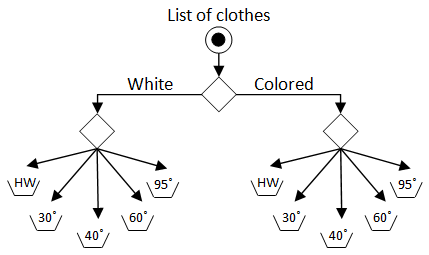
\includegraphics[scale=0.7]{sortingByColorTemp}
	\caption{Sorting algorithm by color and temperature}
	\label{fig:sortingByColorTemp}
\end{figure}

This kind of algorithm is not optimal, nor is it optimized. Of course if time is not an important factor, then clothes from the bin should be washed when bin is full.

\subsubsection{Sorting algorithm using configurable parameters}

Laundry institutions, are very similar to each other when it comes to sorting clothes, but they are not exactly the same. They may have different sized washing machines, the other washes at a higher temperature and all of them have distinct criteria. Meeting the different needs is accomplished by having a flexible system, and software which satisfies all user requirements. \\  The presented software is based on the C\# language, software consists of two parts: configuration and sorting algorithm. Configuration part is finished, however the sorting algorithm is not finished. Purpose of the configuration is to save and load sorting criteria created by user. 
\\
Fabric is sorted by priorities; more sensitive clothes have more privileges than low priority clothes. Same color and same washing temperature clothes could have different priorities, for instance if one clothe is wool and another is synthetic, so synthetic is (possible) lower priority than wool and should be washed using the wool laundry settings. Clothes of the lower priority is washed using higher priority settings and highest priority clothes is washed, according to its label. Figure \ref{fig:sortingByColorTemp} (left) presents an example of configured priorities. \\ Most significant clothes are in the top of list (\textbf{example}: Cotton: Hand wash: 95, Wool: Degree 30: 90),  have the highest priority and the least significant are lowest in the list. 
\\
Different institutions have different washing machine sizes, and all of them during one washing cycle want to utilize the machine to its maximum, making the machine as efficient as possible. Therefore there has been included parameters like total washing machine size and each clothe size, shown on figure \ref{fig:sortingByColorTemp} (right). Total washing machine size defines the threshold (in this case 87\%), which defines when it is not optimal to wash. In other words, washing machine utilization below 87\% is not optimal and cannot be washed. Another configuration of size is how many units of particular type of clothe can fit in one washing machine. For instance in one washing machine can fit 30 shorts (Shorts: 30), so size of the shorts is approximately $\frac{1}{30}$ or utilization of washing machine is about 3.33 \%. So minimum number of the same unit size can be:$\frac{87\%}{3.33\%}\approx 26$. This is what the size of the particular clothe in the database is describing. When the clothes are added to the database they will be attached with a clothe type, that can be enumerated as a size value, this size value can be used for future optimizations of the sorting algorithm.  \\ 

\begin{figure}[h]
	\centering
		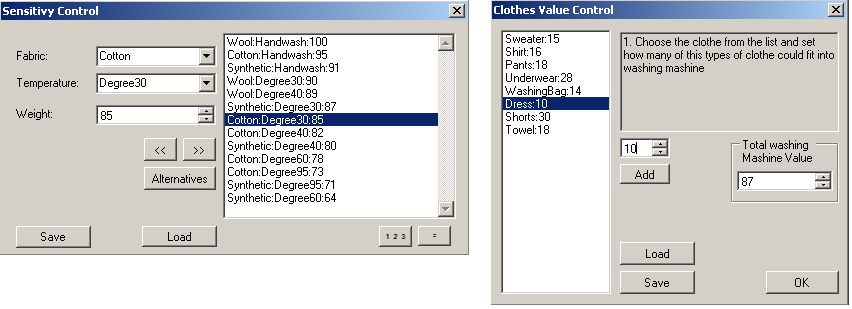
\includegraphics[scale=0.5]{sortinControls}
	\caption{Left: clothes sensitive control; Right: clothes value control}
	\label{fig:sortinControls}
\end{figure}

\begin{figure}[h]
	\centering
		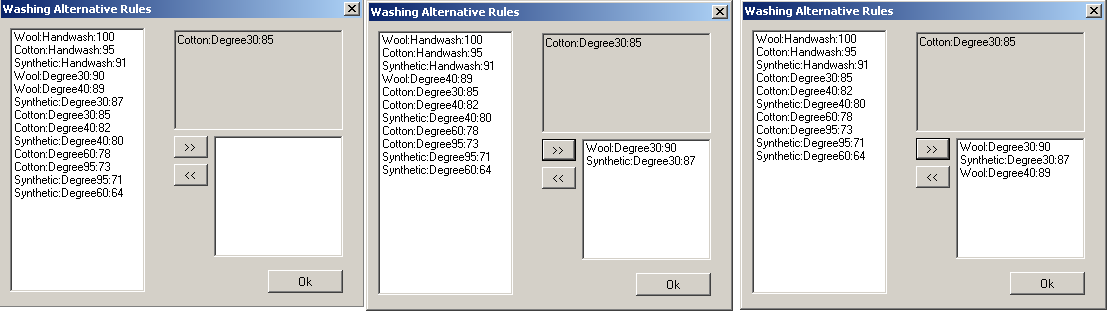
\includegraphics[scale=0.5]{alternativeRules}
	\caption{Washing alternative rules}
	\label{fig:alternativeRules}
\end{figure}

Washing alternatives, what to do when clothe can not be washed in particular case. Figure \ref{fig:sortinControls} presents alternatives of cotton: 30 degree. Shown of the figure this kind of clothe can be washed with the wool: 30 degree (plan B) or Synthetic: 30 degree (plan C) or wool: 40 degree (worst plan if before two does not fit). Each piece of clothes could have any size of plans. All above mentioned parameters can be saved, loaded or updated for the next time use. As shown many features provides quite wide range of washing possibilities.
\\
Further presented sorting algorithm is shown in figure \ref{fig:alternativeRules}. There are four parts (Init, I, II, III) describing the algorithm in a more abstract level. There is one input for incoming clothes and three outputs for outgoing results of the sort. Incoming clothes have parameters like: color, washing temperature, clothe type and fabric and result is a bin designated to current clothe.  Let us explain those four parts in more detail:

\begin{itemize}
	\item 3. Init – all incoming clothes sorted by color and washing temperature. By default all clothes get bin ids and calculated current state. Current state – defines if it is sorted efficiently.
	\item 4. I – check for success. That part check is current state is efficient. If it is than algorithm stops, or emerge time out.
	\item 5. II – try to move clothes from rest to reserve, using washing alternative rules. 
	\item 6. III – try to decrease number of clothes. For example at the table \ref{tab:currentState} rows two and nine utilization is the same 818\%, however efficiency is different. One uses 8 bins and is not efficient, another passes then uses 9 bins (times to be washed).
\end{itemize}

\begin{figure}[h]
	\centering
		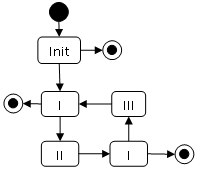
\includegraphics[scale=1]{sortingAlgorithm}
	\caption{Sorting algorithm}
	\label{fig:sortingAlgorithm}
\end{figure}

The algorithms loops;  I, II, I, III, I... while the efficiency is not greater than 87\% (like set in configuration). By default if there are no configurations set, then algorithm works like presented in above chapter (sorting by color and temperature).

\begin{table}[h]
	
    \begin{tabular}{ | p{0.4cm} | p{1cm} | p{2cm} | p{1.7cm} |p{2cm} |p{1cm} |p{1.3cm} |p{1.2cm} |p{1.3cm} |}
    \hline
	Bin Id & Color & Washing Temperature & TotalBin Utilization (TBU) & NumberOf Bins Require (NBR) & Rest & Efficiency & Reserve & Success\\ \hline
	1 & White & 95 & 448\% & 4 & 48\% & 48\% & 52 \% & Fail \\ \hline
	2 & White & 60 & 818\% & 8 & 18\% & 18\% & 82 \% & Fail \\ \hline
	3 & White & 40 & 89\% & 1 & 0\% & 89\% & 11 \% & Pass \\ \hline
	4 & White & 30 & 639\% & 6 & 39\% & 39\% & 61 \% & Fail \\ \hline
	5 & White & HW & 159\% & - & - & - & - & - \\ \hline
	6 & Colored & 95 & 698\% & 7 & 0\% & 99\% & 2 \% & Pass \\ \hline
	7 & Colored & 60 & 2110\% & 21 & 10\% & 10\% & 90 \% & Fail \\ \hline
	8 & Colored & 40 & 788\% & 8 & 0\% & 98.5\% & 1.5 \% & Pass \\ \hline
	9 & Colored & 30 & 818\% & 9 & 0\% & 90.8\% & 9.2 \% & Pass \\ \hline
	10 & Colored & HW & 420\% & - & - & - & - & - \\ \hline
	11 & ... & ... & ... & ... & ... & ... & ... & ... \\ \hline
	- & - & - & - & - & - & Total: 62.54\% & - & All: No \\ \hline
    \end{tabular}
	\caption{Example of current state (when: Total washing machine value 87 \%)}
	\label{tab:currentState}
\end{table}

\newpage

Current state of the sorting is represented by table \ref{tab:currentState} where all values mutate and adjust during sorting. Quantity of incoming clothes set bin ids and total bin utilization (TBU). TBU defines how many times it is needs to be washed, and is calculated by formula 1:

\begin{equation}
TBU=ClotheType1\cdot K1+ClotheType2\cdot K2+...+ClotheType(n)\cdot K(n) \label{eq:eq1}
\end{equation}

Where clothe type can be: Sweater, Shirt, Pants, Underwear, WashingBag, Dress, Shorts, Towel and BedLinen. 
\\
Clothes coefficients: k1,k2,k3,...k(n) set by clothes value control.
Calculation of how many number of bins require (NBR) done by formula 2:  

\begin{equation}
NBR=\frac{TBU}{100\%},\textrm{Round by 87\%} \label{eq:eq2}
\end{equation}

Rest calculated by:

\begin{equation}
Rest=TBU-NBR\cdot 100\% \label{eq:eq3}
\end{equation}

When the results are negative than there is no rest, else rest is necessary. Rest means how many percent of clothes left and can not be washed, because of a to small amount. So rest can be zero or lesser than 87 \%, because greater then 87\% indicates smaller entity which can be washed.
\\
Efficiency can be calculated considering rest, diagram shown in figure \ref{fig:efficiencyCalculation}. Efficiency describes is there cost-efficiency to wash or not. Wash is done when the cost efficiency is greater then 87\%.

\begin{figure}[h]
	\centering
		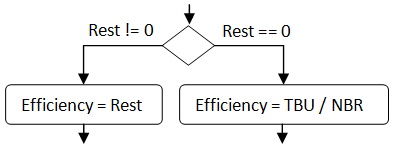
\includegraphics[scale=0.7]{efficiencyCalculation}
	\caption{Efficiency calculation diagram}
	\label{fig:efficiencyCalculation}
\end{figure}

Incoming clothes are taken one after another and moved to the particular bin. If there are no clothes left then the algorithm checks how many bins are required. If there are more than zero bins then the current state is calculated and set, like shown in the table \ref{tab:currentState}. Once all the clothes and bins have been set and there is nothing left then the algorithm has ended. \newpage

\begin{figure}[h]
	\centering
		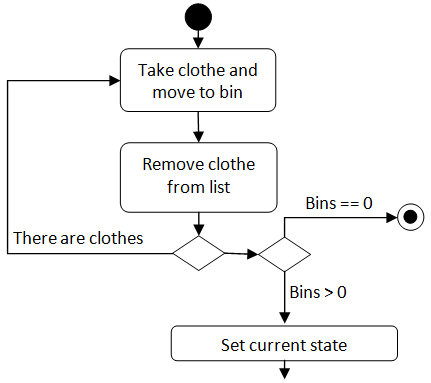
\includegraphics[scale=0.7]{diagramInit}
	\caption{Diagram Init}
	\label{fig:planning}
\end{figure}

The algorithm checks for success and for time-out, figure \ref{fig:diagramI}. If all bins have greater efficiency than 87\% then the current state is satisfied and the clothes can be washed, else there is a time-out, and the algorithm also stops. Purpose of the time-out is to avoid a infinite loop.

\begin{figure}[h]
	\centering
		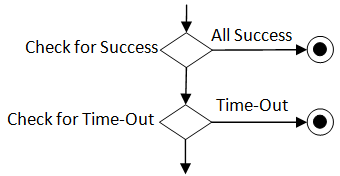
\includegraphics[scale=0.7]{diagramI}
	\caption{Diagram I}
	\label{fig:diagramI}
\end{figure}

Last two part (II and III) are very similar. Both of them try change the current state estimate and compare with previous state, improving efficiency. If new state is better than previous then state is set to current, else the last state is kept.  \newpage

\begin{figure}[h]
	\centering
		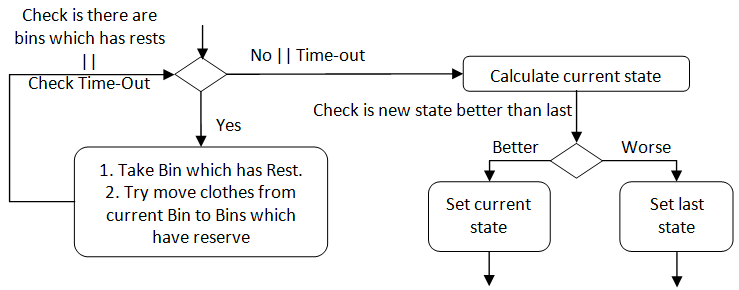
\includegraphics[scale=0.5]{diagramII}
	\caption{Diagram II}
	\label{fig:diagramII}
\end{figure}

The figure \ref{fig:diagramI} of the sorting algorithm is changing the current state by moving clothes from bins which have rests to bins which have reserves, if result is an improvement then new state is set to current state. 

\begin{figure}[h]
	\centering
		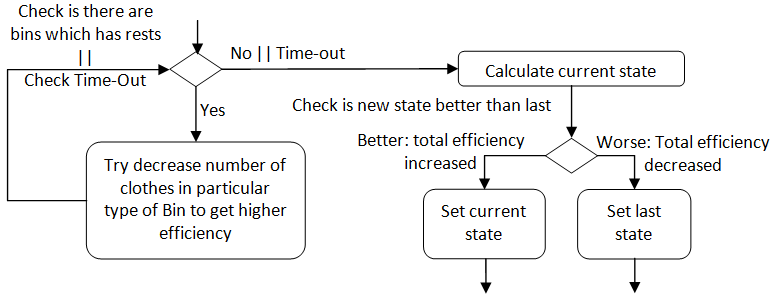
\includegraphics[scale=0.5]{diagramIII}
	\caption{Diagram III}
	\label{fig:diagramIII}
\end{figure}
There are concurrency between II and III, if something changes at II then III can also possibly change and vice versa.
\\
The figure \ref{fig:diagramII} of the sorting algorithm change the number of clothes in particular type of bin. For instance the quantity of 818\% gives result for 8 bins and 18\% rest. However efficiency of 8 bins is 100\% and for the last one is only 18\%. Eight bins can be washed and the last must rest and should wait. If 818\% of clothes we wash by 9 bins then we get efficiency of 90.8\% and reserve 9.2\%. This would be optimal and new state is set.

\subsection{Future Work}
